\documentclass[10pt]{beamer}

\usetheme{metropolis}
\usepackage{appendixnumberbeamer}

\usepackage{booktabs}
\usepackage[scale=2]{ccicons}
\usepackage{graphicx}
\usepackage{hyperref}
\usepackage{circuitikz}
\usepackage{pdflscape}
\usepackage{smartdiagram}

\usepackage{color}
\usepackage{listings}

\lstset{
	basicstyle=\footnotesize\ttfamily,
    keepspaces=true,
    showstringspaces=false,
    language=PHP,
    commentstyle=\ttfamily,
}

\usepackage[OT4]{polski}
\usepackage[utf8]{inputenc}

\usepackage{pgfplots}
\usepgfplotslibrary{dateplot}

\usepackage{xspace}
\newcommand{\themename}{\textbf{\textsc{metropolis}}\xspace}

\setbeamertemplate{frame footer}{}
\setbeamertemplate{frame numbering}{}

\usetikzlibrary{shapes,arrows}

\tikzstyle{decision} = [diamond, draw, fill=blue!20, 
    text width=4.5em, text badly centered, node distance=3cm, inner sep=0pt]
\tikzstyle{block} = [rectangle, draw, fill=blue!20, 
    text width=5em, text centered, rounded corners, minimum height=4em]
\tikzstyle{line} = [draw, -latex']
\tikzstyle{cloud} = [draw, ellipse,fill=red!20, node distance=3cm,
    minimum height=2em]


\title{Czysty kod, część I}

\subtitle{Projektowanie i programowanie systemów internetowych I}
\author{mgr inż. Krzysztof Rewak}
\date{\today}
\institute{Wydział Nauk Technicznych i Ekonomicznych \\ Państwowa Wyższa Szkoła Zawodowa im. Witelona w Legnicy}

\begin{document}

\maketitle

\begin{frame}{Plan prezentacji}
  \setbeamertemplate{section in toc}[sections numbered]
  \tableofcontents[hideallsubsections]
\end{frame}


\section{Czysty kod}

\begin{frame}{Czysty kod}
	Czym jest \emph{czysty kod}?
\end{frame}

\begin{frame}{Bjarne Stroustrup}
	\emph{Lubię, gdy mój kod jest \textbf{elegancki} i \textbf{efektywny}.}
	
	\emph{Logika kodu powinna być \textbf{prosta}, aby nie mogły się w niej kryć błędy; zależności minimalne dla uproszczenia utrzymania; obsługa błędów kompletna zgodnie ze zdefiniowaną strategią; a wydajnośc zbliżona do optymalnej, aby nikogo nie \textbf{kusiło} psucie kodu w celu wprowadzenie niepotrzebnych optymalizacji.}
	
	\emph{Czysty kod wykonuje dobrze jedną operację.}
\end{frame}

\begin{frame}{Dave Thomas i Andy Hunt}
	Kod jest jak budynek.
	
	\emph{Budynek z rozbitymi oknami wygląda, jakby nikt się o niego nie \textbf{troszczył}. Dlatego inni ludzie również przestają się o niego troszczyć. W ten sposób coraz więcej okien jest rozbijanych. W końcu sami je rozbijają. Zaczynają bazgrać na fasadzie i pozwalają na powstanie gór śmieci.}
	
	\emph{Jedno rozbite okno rozpoczyna \textbf{proces upadku}.}
\end{frame}

\begin{frame}{Grady Booch}
	\emph{Czysty kod jest prosty i bezpośredni. Czysty kod \textbf{czyta się} jak dobrze napisaną prozę. czysty kod nigdy nie zaciemnia zamiarów projektanta; jest pełen \textbf{trafnych abstrakcji} i \textbf{prostych ścieżek sterowania}.}
\end{frame}

\begin{frame}{Dave Thomas}
	\emph{Czysty kod może być \textbf{czytany} i rozszerzany przez \textbf{innego programistę} niż jego autor. Posiada on \textbf{testy} jednostkowe i akceptacyjne. Zawiera \textbf{znaczące} nazwy. Oferuje jedną, a nie wiele ścieżek wykonania jednej operacji. Posiada minimalne zależności, które są jawnie zdefiniowane, jak również zapewnia jasne i \textbf{minimalne} API. Kod powinien być \textbf{opisywany} przy jednoczesnej zależności od języka - nie wszystkie potrzebne informacje mogą być wyrażane bezpośrednio w kodzie.}
\end{frame}

\begin{frame}{Michael Feathers}
	\emph{Mógłbym wymieniać wszystkie cechy, jakie zauważam w czystym kodzie, ale istnieje jedna, która prowadzi do pozostałych. Czysty kod zawsze wygląda, jakby był napisany przez kogoś, komu na nim \textbf{zależy}. Nie ma w nim nic oczywistego, co mógłbyś poprawić.}
	
	\emph{Autor kodu pomyślał o wszystkim i jeżeli próbujemy sobie wyobrazić usprawnienia, prowadzą one nas tam, skąd zaczęliśmy, co pozwala nam \textbf{docenić} kod, który ktoś dla nas napisał - kod, który napisał ktoś, kto naprawdę przyjmuje się swoimi zadaniami.}
\end{frame}

\begin{frame}{Ward Cunningham}
	\emph{Wiemy, że pracujemy na czystym kodzie, jeżeli każda procedura okazuje się taką, \textbf{jakiej się spodziewaliśmy}. Można nazywać go również pięknym kodem, jeżeli wygląda, jakby ten język został stworzony do rozwiązania danego problemu.}
\end{frame}

\section{Nomenklatura}

\begin{frame}{Sensowne nazywanie}
	\emph{Wybór odpowiedniej nazwy to dobra inwestycja.}
\end{frame}

\begin{frame}{Sensowne nazywanie}
	Każda nazwa zmiennej, funkcji, argumentu, klasy czy interfejsu powinna być przemyślana oraz powinna przedstawiać intencję.
\end{frame}

\begin{frame}
	\begin{figure} \centering
		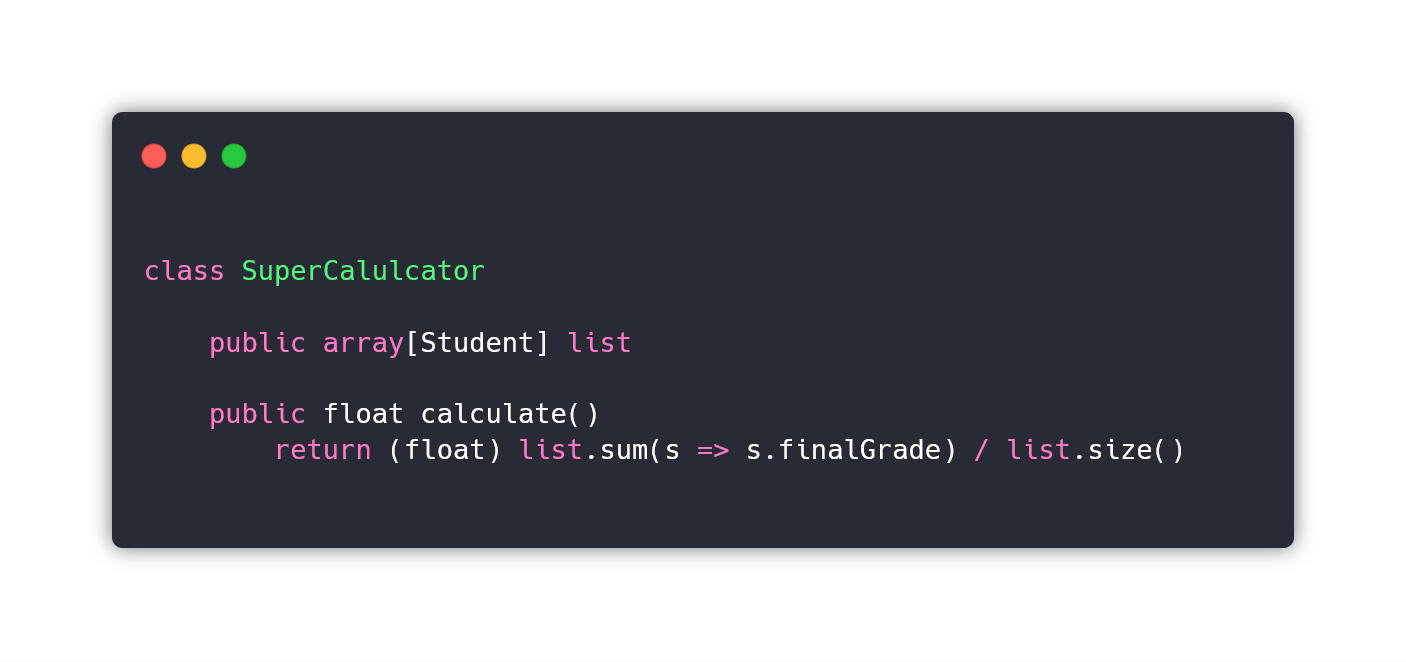
\includegraphics[width=\textwidth]{names.png}
	\end{figure}
\end{frame}

\begin{frame}{Sensowne nazywanie}
	Czasami nazwiemy zmienne inaczej niż \texttt{a} i \texttt{b}, ale i tak wiele nam to nie pomoże. Nazwy powinny idealnie odzwierciedlać swoje przeznaczenie i nie generować niepewności.
\end{frame}

\begin{frame}
	\begin{figure} \centering
		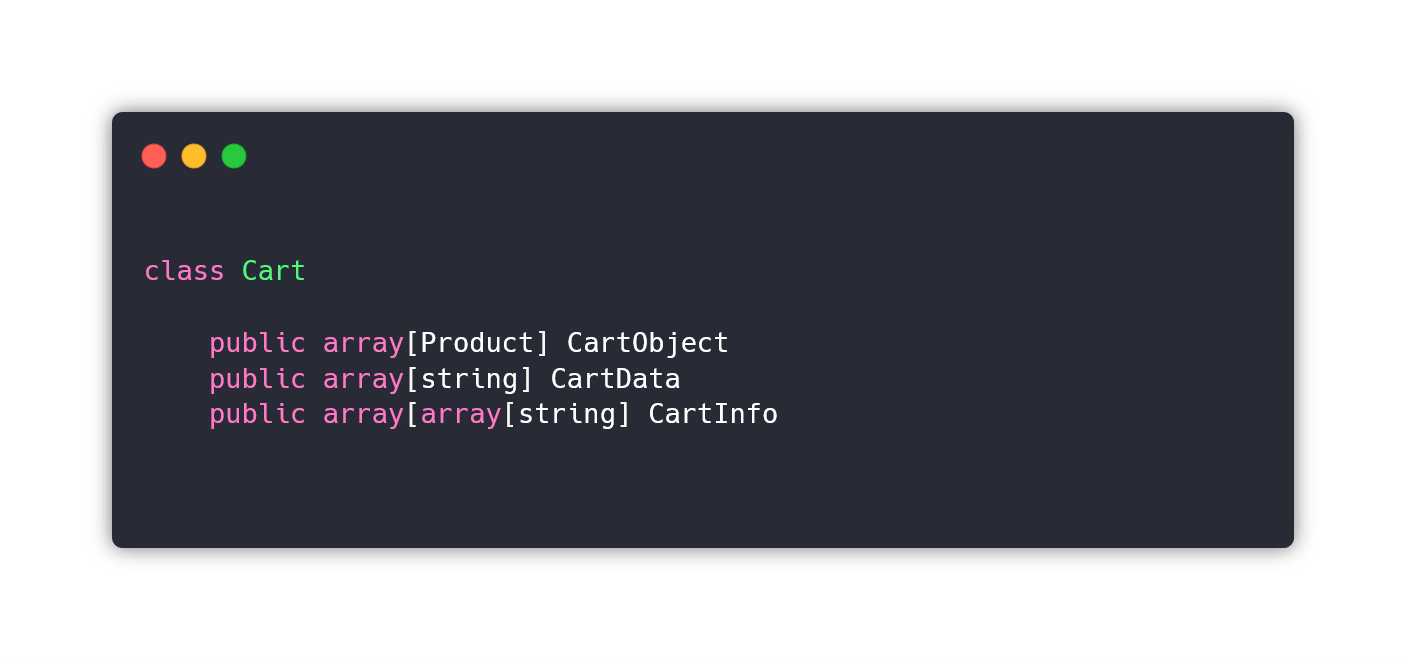
\includegraphics[width=\textwidth]{useless.png}
	\end{figure}
\end{frame}

\begin{frame}{Zakaz dezinformacji}
	Dezorientacja może występować w kodzie na kilka sposobów.
\end{frame}

\begin{frame}
	\begin{figure} \centering
		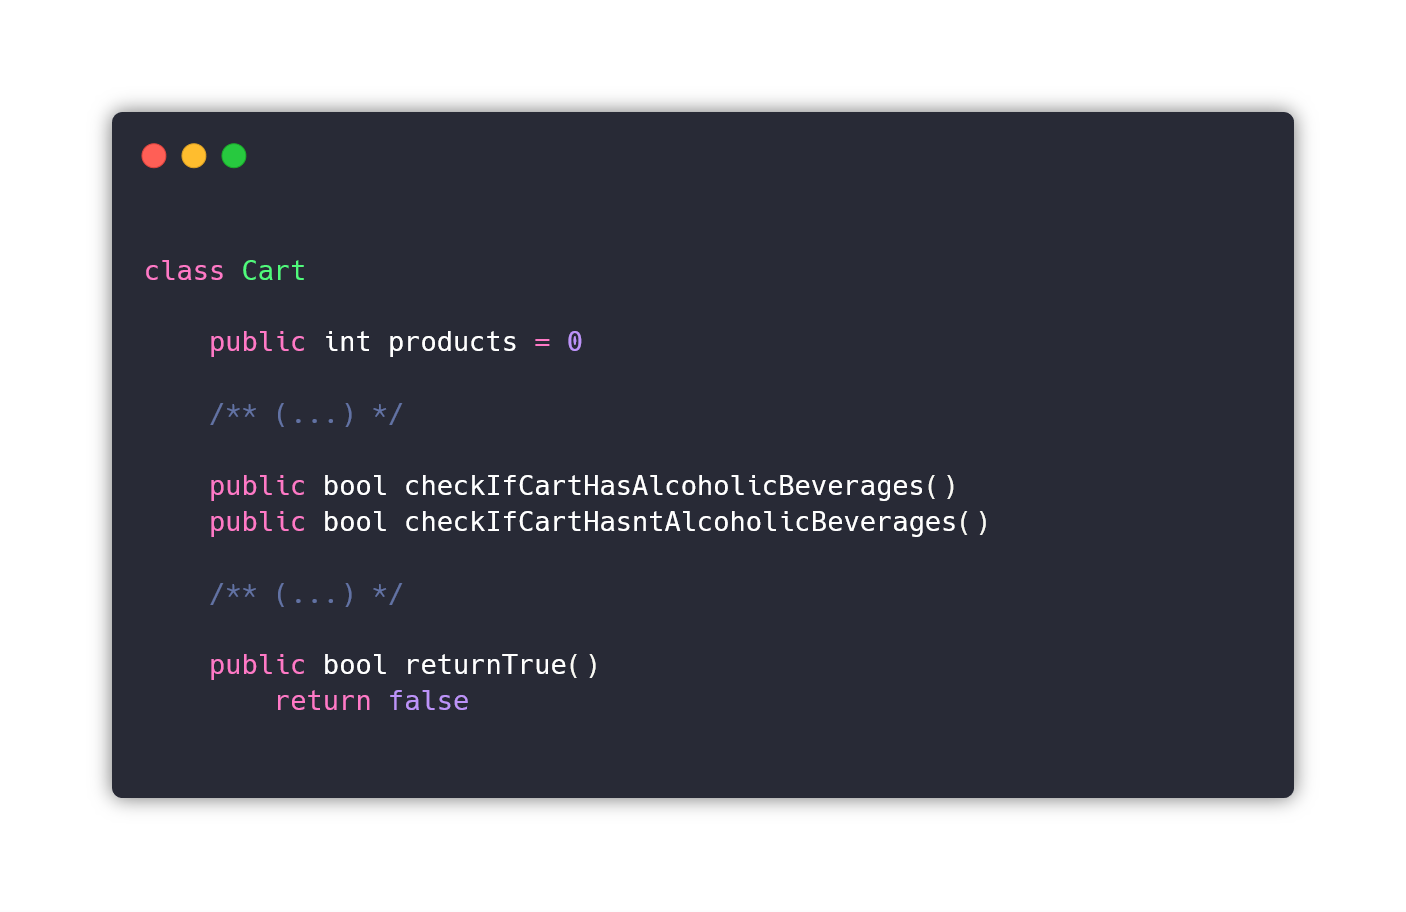
\includegraphics[width=\textwidth]{dezinfo.png}
	\end{figure}
\end{frame}

\begin{frame}{Nie koduj}
	Kod nie powinien też zawierać w sobie żadnych zbędnych informacji.
	
	Przykładowo dawniej popularna notacja węgierska jest obecnie coraz rzadziej używana ze względu na swoją redundancję.
\end{frame}

\begin{frame}
	\begin{figure} \centering
		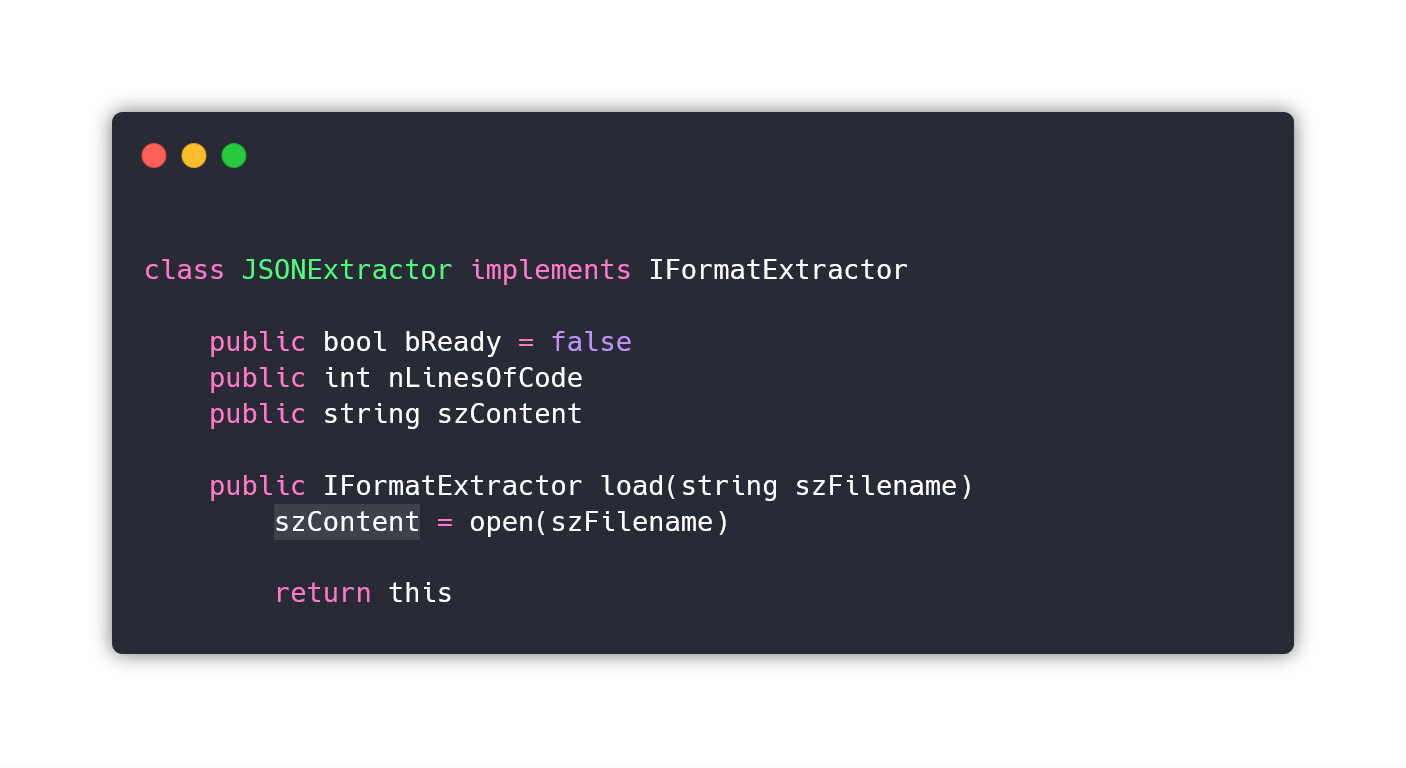
\includegraphics[width=\textwidth]{hn.png}
	\end{figure}
\end{frame}

\begin{frame}{Nie kombinuj}
	Słowa mają swoje synonimy, jednak powinniśmy używać ich z głową. Lepiej wybrać jedno słowo i się go trzymać wewnątrz projektu czy żonglować w co drugiej klasie różnymi nazwami?
\end{frame}

\begin{frame}
	\begin{figure} \centering
		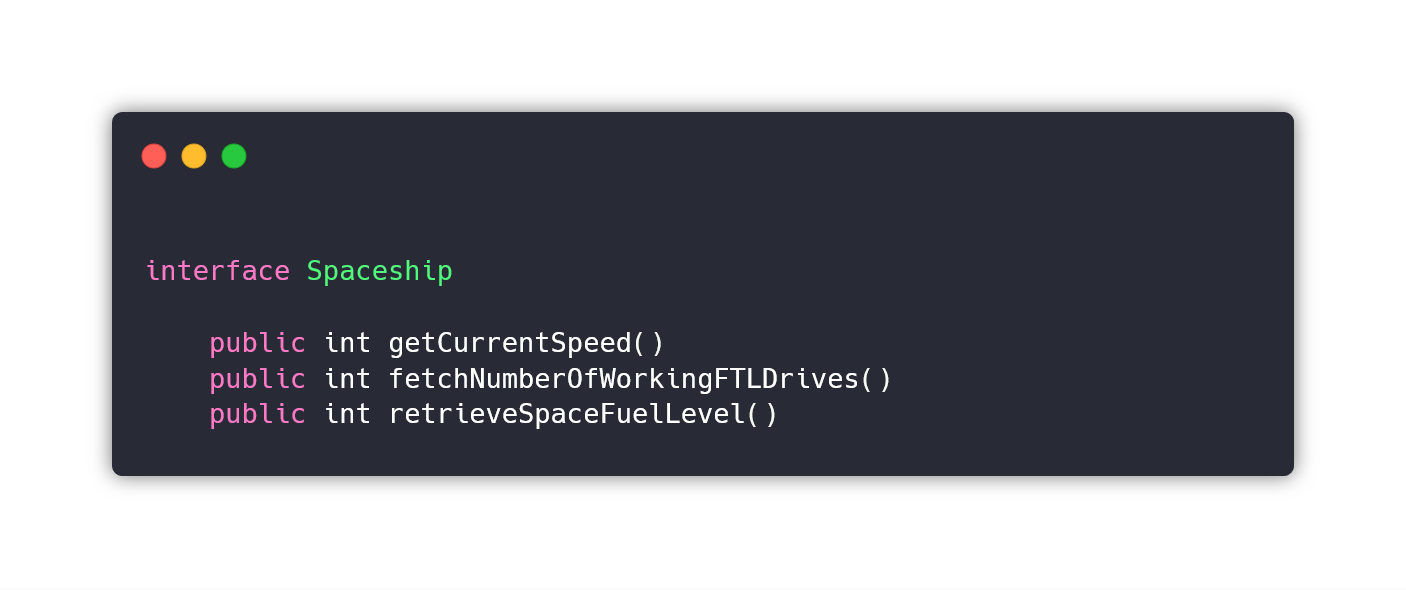
\includegraphics[width=\textwidth]{gets.png}
	\end{figure}
\end{frame}

\section{Komentarze}

\begin{frame}{Brian W. Kernighan i P.J. Plaugher}
	\emph{Nie komentuj złego kodu - popraw go.}
\end{frame}

\begin{frame}{Komentarze}
	\emph{Obecność komentarzy zawsze sygnalizuje nieporadność programisty.}
\end{frame}

\begin{frame}{Komentarze}
	Komentarz może być przydatnym narzędziem, niestety najczęściej jest przeszkodą w tworzeniu dobrego kodu.
\end{frame}

\begin{frame}
	\begin{figure} \centering
		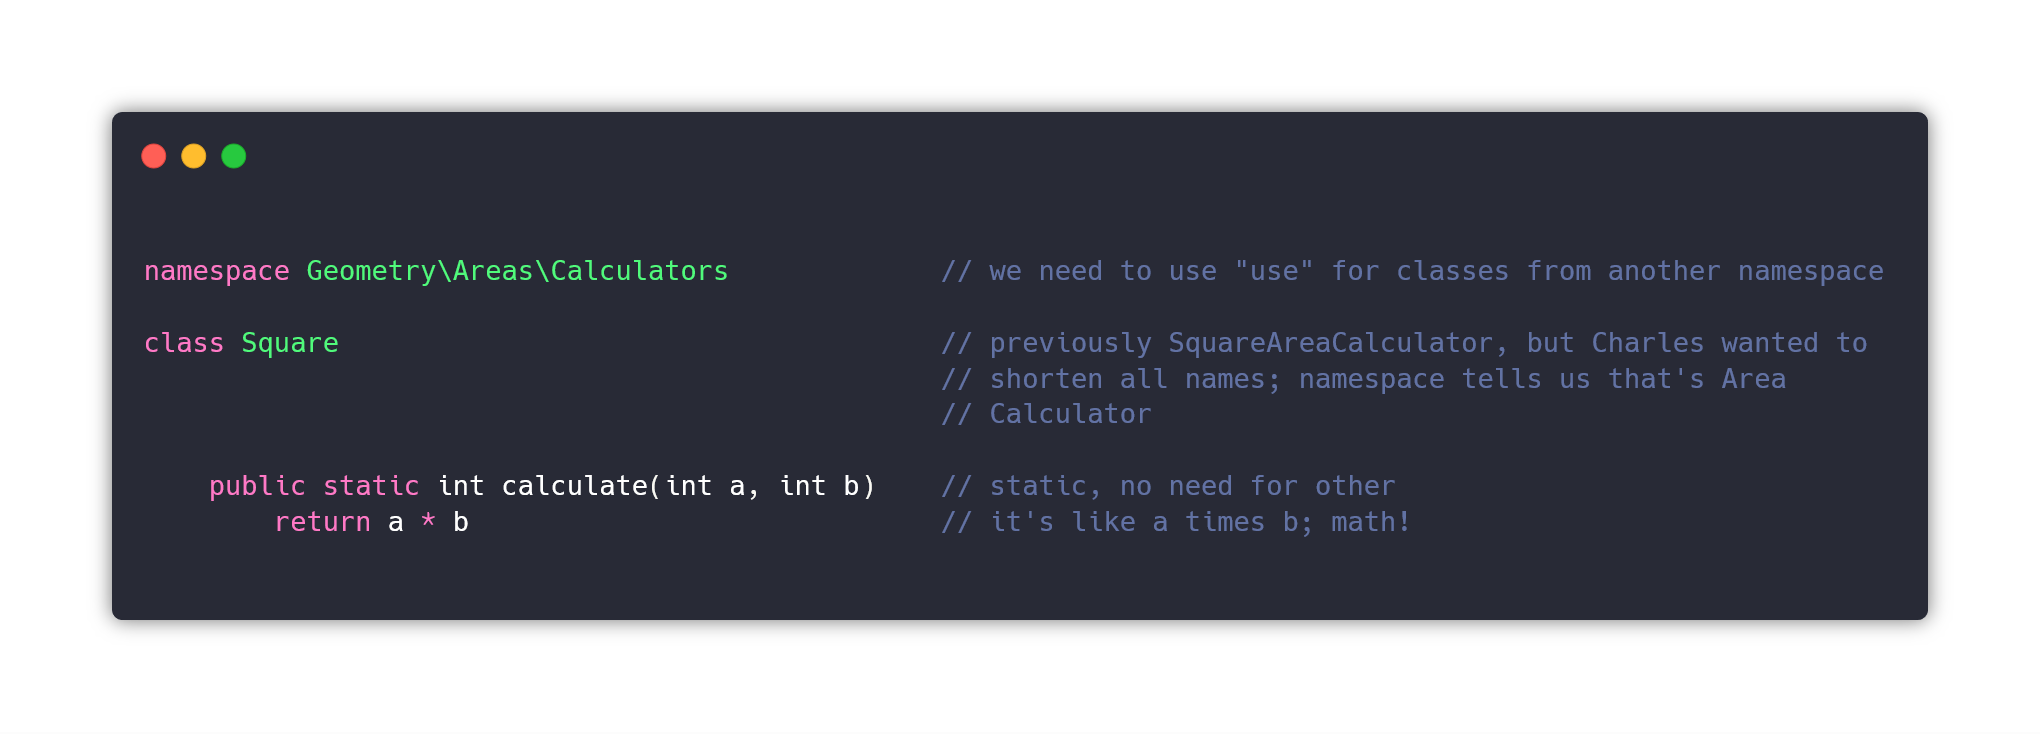
\includegraphics[width=\textwidth]{oe.png}
	\end{figure}
\end{frame}

\begin{frame}
	\begin{figure} \centering
		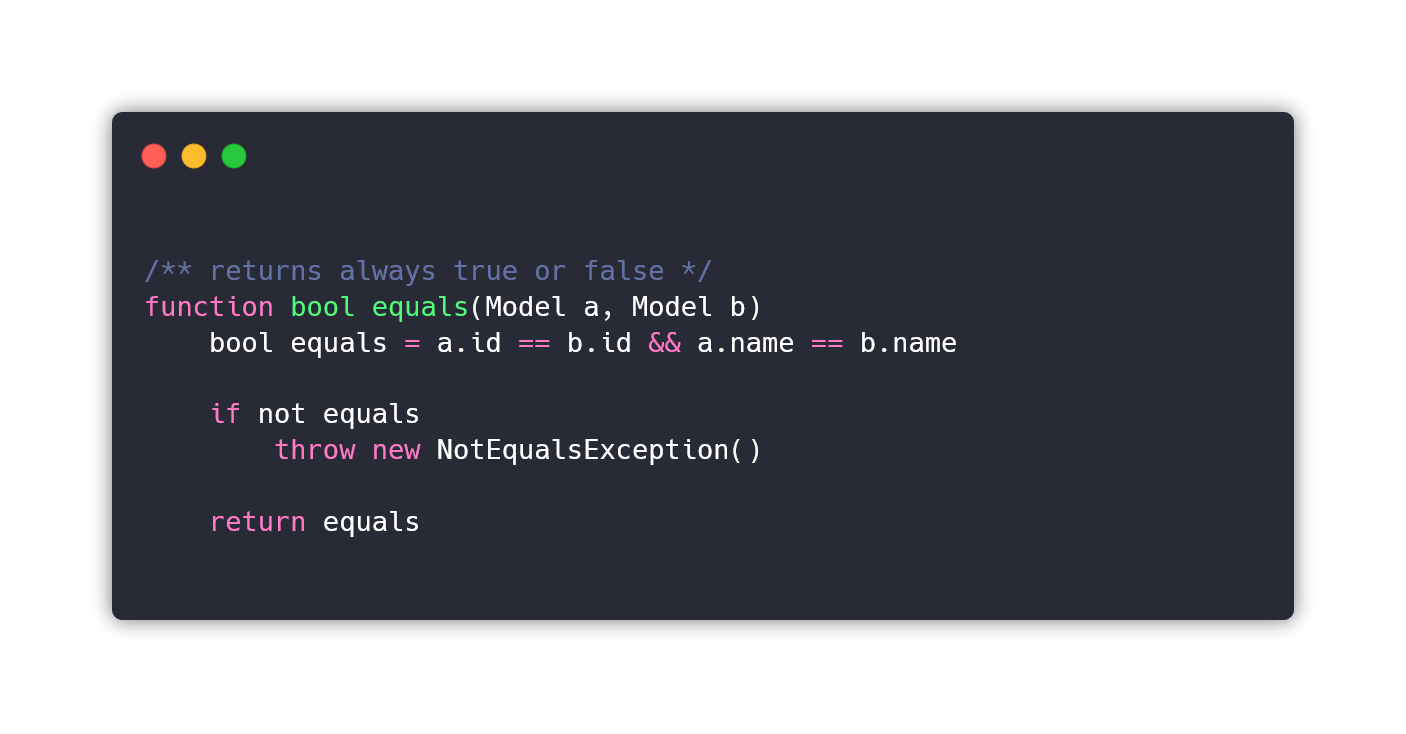
\includegraphics[width=\textwidth]{lie.png}
	\end{figure}
\end{frame}

\begin{frame}
	\begin{figure} \centering
		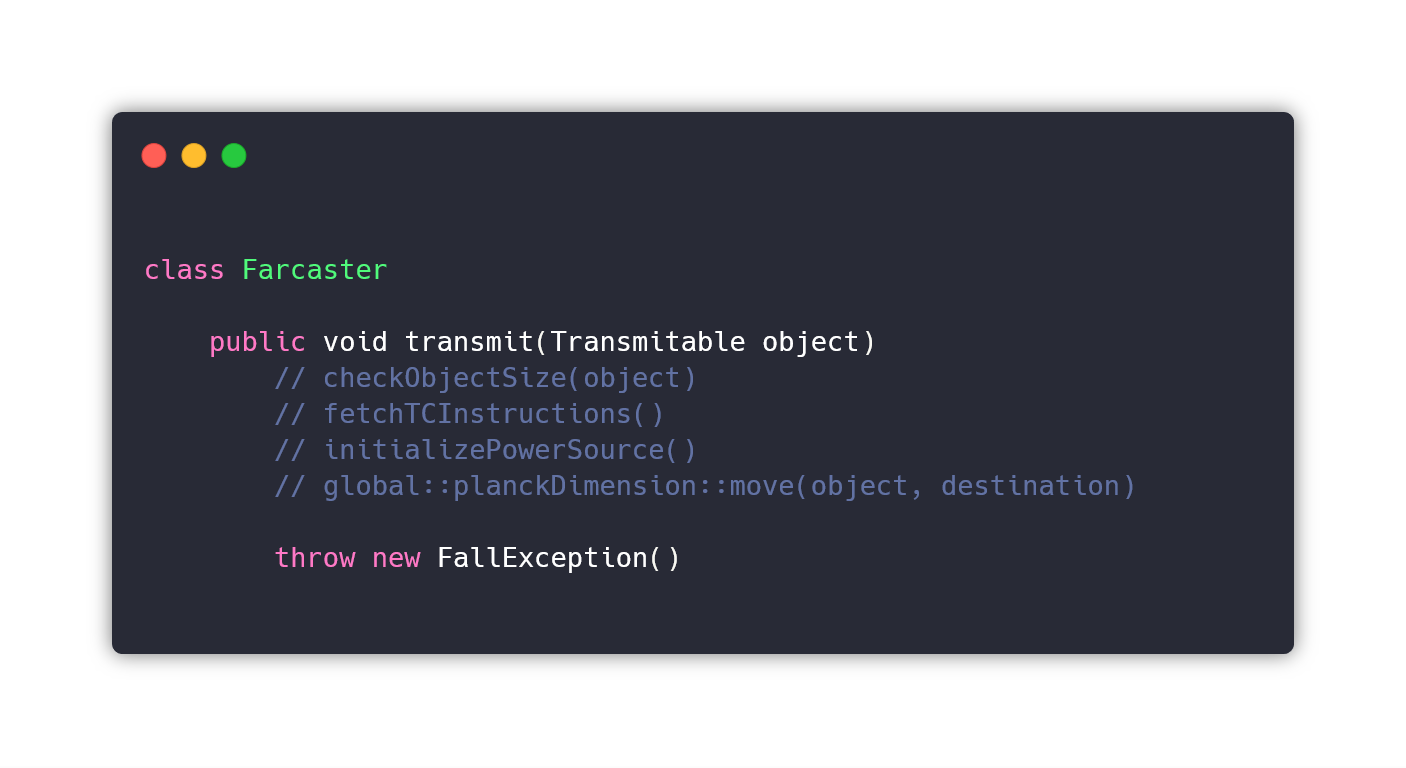
\includegraphics[width=\textwidth]{farcaster.png}
	\end{figure}
\end{frame}

\begin{frame}{Komentarze}
	Czasami komentarz przetrzymuje dodatkowe informacje. Ale czy warto go używac?
\end{frame}

\begin{frame}
	\begin{figure} \centering
		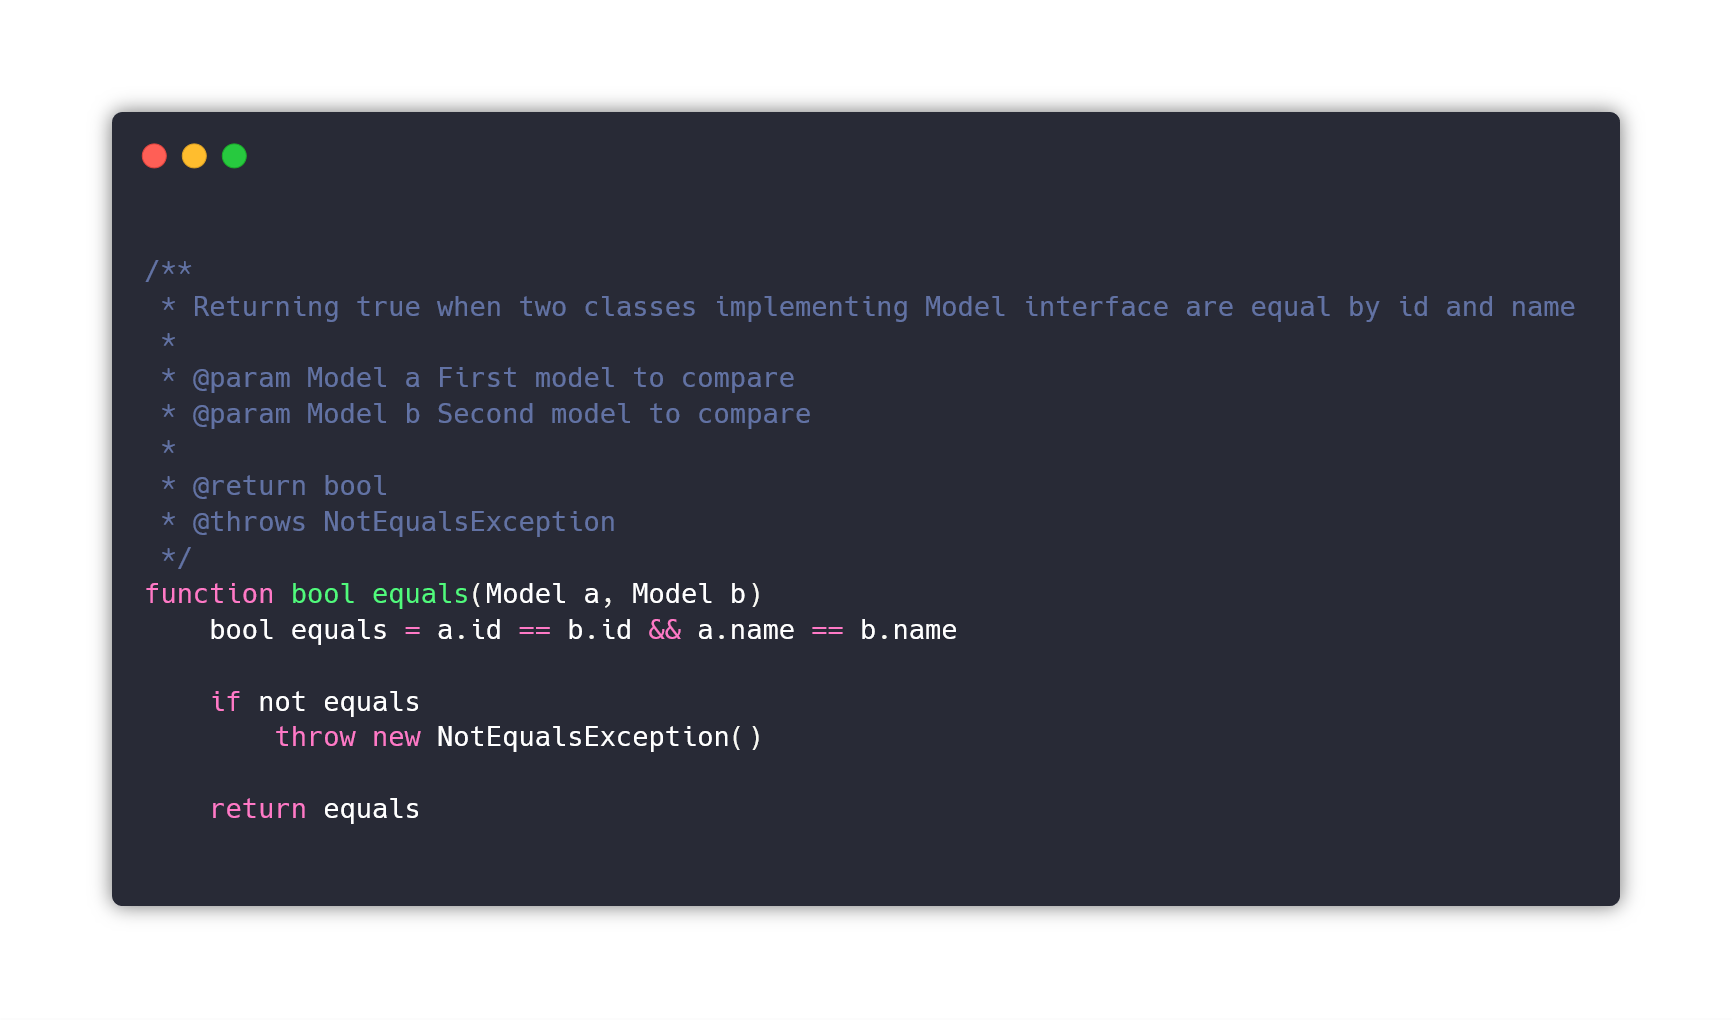
\includegraphics[width=\textwidth]{docs.png}
	\end{figure}
\end{frame}

\begin{frame}
	\begin{figure} \centering
		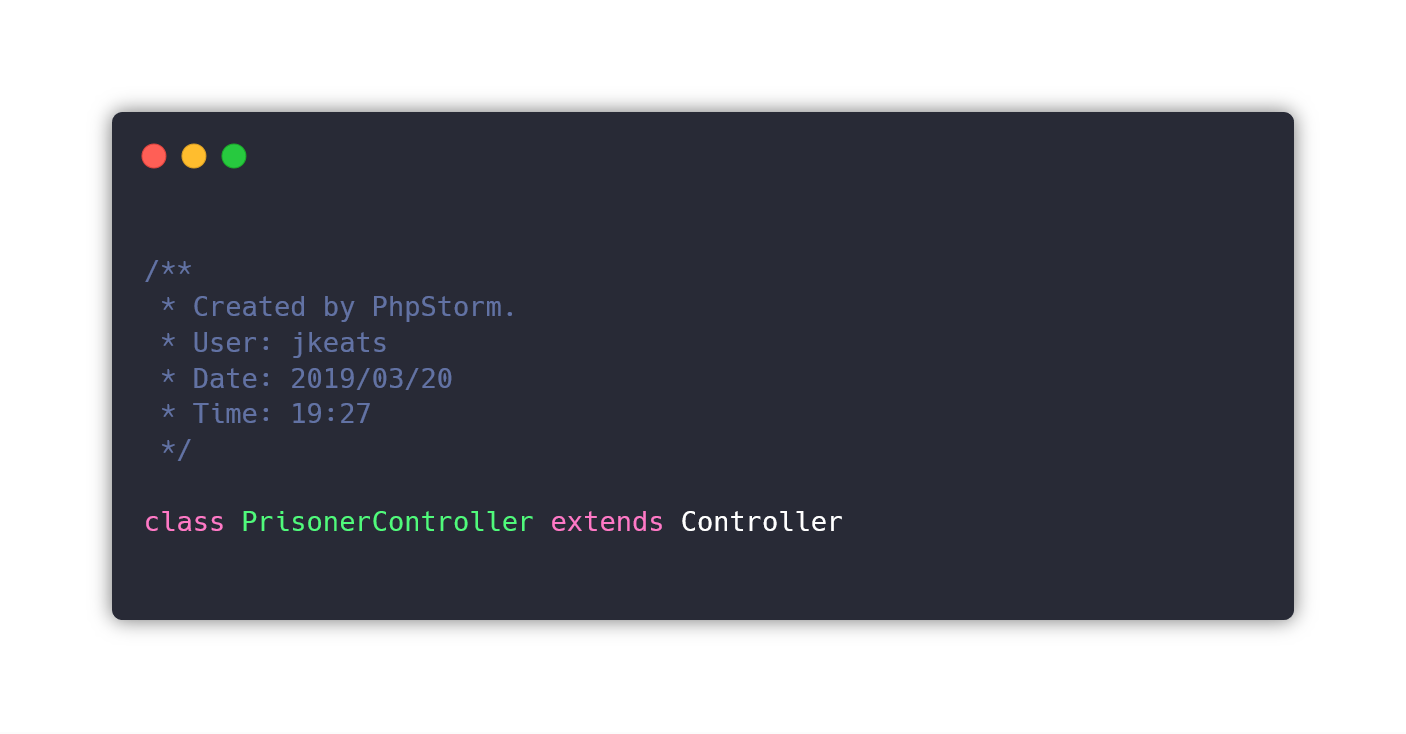
\includegraphics[width=\textwidth]{signatures.png}
	\end{figure}
\end{frame}

\begin{frame}{Komentarze}
	Zatem kiedy korzystać z komentarzy?
\end{frame}

\begin{frame}{Komentarze}
	\begin{itemize}
		\item do informacji o prawach autorskich, jeżeli musimy takie informacje zawrzeć?
		\item do wyjaśnienia trudnych rzeczy?
		\item do oznaczenia TODO?
	\end{itemize}
\end{frame}

\section{Podsumowanie}

\appendix

\begin{frame}[standout]
	Pytania?
\end{frame}

\begin{frame}{}

	Kod prezentacji dostępny jest w repozytorium git pod adresem \texttt{https://bitbucket.org/krewak/pwsz-ppsi} \\ \ \\

	\begin{figure}
		\centering
		\href{https://bitbucket.org/krewak/pwsz-ppsi}{
			
\includegraphics[width=.15\textwidth]{../_template/bitbucket.png}
		}
	\end{figure}
	
	Wszystkie informacje dot. kursu dostępne są pod adresem \texttt{http://pwsz.rewak.pl/kursy/4} \\ \ \\

	\begin{figure}
		\centering
		\href{http://pwsz.rewak.pl/kursy/3}{
			
\includegraphics[width=.15\textwidth]{../_template/rewak.png}
		}
	\end{figure}

\end{frame}

\end{document}
